\documentclass[12pt]{article}

\usepackage[symbol,perpage]{footmisc} %this is for dagger footnotes
\usepackage{xcolor}
\usepackage{hyperref}
\hypersetup{%
  colorlinks=true,% hyperlinks will be coloured
  linkcolor=blue,% hyperlink text will be green
  linkbordercolor=red,% hyperlink border will be red
}

\input quiz-setup
\newcommand{\version}{} 
\newcommand{\xzero}{}
\newcommand{\xone}{}
\newcommand{\xtwo}{}
\newcommand{\xthree}{}
\newcommand{\xfour}{}
\newcommand{\xfive}{}
\newcommand{\vecb}[1]{\mathbf{#1}}

\newcommand{\ExamName}{Quiz \#0\version}
% \newcommand{\CourseName}{Math 34A}
% \renewcommand{\Quarter}{Spring 2017}

%these are for dagger footnotes
\DefineFNsymbols*{daggorath}{{$\dagger$}{$\ddagger$}{$\dagger\dagger$}{$\ddagger\ddagger$}}
\setfnsymbol{daggorath}
\renewcommand{\thefootnote}{\fnsymbol{footnote}}
%\end dagger footnotes stuff




\begin{document}
%%
%% Version A:
\renewcommand{\version}{}
\renewcommand{\xzero}{0.0}
\renewcommand{\xone}{1.3}
\renewcommand{\xtwo}{2.9}
\renewcommand{\xthree}{4.1}
\renewcommand{\xfour}{5.3}
\renewcommand{\xfive}{6.5}
% 
\begin{minipage}{0.25\linewidth}
  \CourseName\ \Quarter \\
  \ExamName \\[1em]
  \textbf{No calculators}\\[2em]
\end{minipage}
\hfill
\begin{minipage}[t]{0.4\linewidth}
  
\begin{tikzpicture}[x=26mm,y=16mm]
    \draw[thick,black] (0,0) rectangle (3,1);
    \node[\faintcolor,right] at (0,0.2) {\large\textsf{PRINT NAME}};
  \end{tikzpicture}
\end{minipage}
\hfill
\begin{minipage}{0.25\linewidth}
  \vspace*{-3.25em}
  \ \hfill
  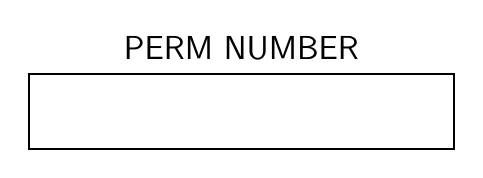
\begin{tikzpicture}[x=36mm,y=16mm]
    \node[\faintcolor] at (0.75,0.8) {\large\textsf{PERM NUMBER}};
    \draw[thick,black] (0,0) rectangle (1.5,0.6);
  \end{tikzpicture}
\end{minipage}
% \medskip
\vspace*{-0.25in}

%Put your answer in the 
%\begin{tikzpicture}[x=10mm,y=10mm,baseline=3mm] 
%  \draw[thick,black] (0,0) rectangle (3,1);
%  \node[\faintcolor] at (1.5,0.4) {\Huge\textsf{box}};
%\end{tikzpicture}
%provided.
\hfill
\begin{minipage}{0.5\linewidth}
\begin{center}

  \textbf{TA:}\ 
  \parbox[t]{0.7in}{%
    \checkbox\ \TAOne \\
    \checkbox\ \TATwo 
  }
  %\parbox[t]{0.7in}{%
  %  \checkbox\ \TAThree\\
  %  \ \ \ 
  %}
  % \ 
  % \parbox[t]{4in}{%
  % \textbf{Section Time:}
  \hfill%\hspace*{0.25in}
  % \ 
  % \parbox[t]{4in}{%
  % \textbf{Section Time:}
  \textbf{Time:}
  \parbox[t]{0.55in}{%
    \checkbox\ 4:30 \\
    \checkbox\ 5:30
  }
  \quad
  \parbox[t]{0.55in}{%
    \checkbox\ 6:30 \\
    \checkbox\ 7:30 
  }
  % }
%  \textbf{TA:}\ 
%  \parbox[t]{0.95in}{%
%    \checkbox\ \TAOne
%  }
%  \parbox[t]{0.95in}{%
%    \checkbox\ \TATwo\\
%  }
%%  \parbox[t]{0.95in}{%
%%    \checkbox\ \TAThree
%%  }
%  \hspace*{0.5in} 
%  \parbox[t]{3in}{%
%    \textbf{Section Time:}
%    \parbox[t]{0.75in}{%
%      \checkbox\ 4:30 \\
%      \checkbox\ 5:30
%    }
%    \parbox[t]{0.75in}{%
%      \checkbox\ 6:30 \\
%      \checkbox\ 7:30
%    }
%  }
\end{center}

\end{minipage}
\noindent\hspace*{-2em}\rule{\textwidth+4em}{1pt}%

\mbox{}

Normally we will be doing all our quizzes ``live" in our Zoom meeting for section. This week we will just be practicing and familiarizing ourselves with submitting to Gradescope.

\mbox{}

\textbf{Download and read the document ``Submitting PDF homework in Gradescope" from the Gaucho-Space page, and read it. Yes, actually read it. Then answer the following questions about what you read: }

\begin{enumerate}
  \setcounter{problemnumber}{0}
\Problem Download the app which is recommended for your device. Which app did you download?
\vfill

\Problem We always scan our documents into pdf format so that Gradescope will play nice with our files and not make our TAs go prematurely gray. The answer to this question is ``I will always submit my work as a pdf, never jpg or anything else." Please write the answer to this question. 
\vfill

\Problem Once you've scanned every page of your document, what should you \textbf{always} do before you send it?
\vfill

\Problem How do you get the scan from your phone or tablet to your computer?
\vfill

\pagebreak


\textbf{If you have an iPad or other tablet, it's a great idea to import your quizzes into your favorite note-taking app and write directly on the quiz.} This is easier for everyone, and it means the above four questions won't really apply to you. (You still have to answer them though.)
\textbf{Most importantly, make sure you know how to export your quiz as a PDF.} 
\href{https://support.gingerlabs.com/hc/en-us/articles/205228298-Exporting-Notes}{[How to do it in Notability]} 
\href{https://support.goodnotes.com/hc/en-us/articles/360000630495-How-to-export-documents-or-pages-in-GoodNotes-5}{[How to do it in GoodNotes 5]}

\mbox{}

\textcolor{blue}{\textbf{Do not write the following problems on the same page as problems 1-4.}}

\Problem True or False: If Gradescope gives you an option to submit your file as a JPG or a PDF, then either one is fine. 
\vspace*{24pt}
	
\Problem Suppose you upload your document and you are taken to a page that asks you to assign questions and pages. What do you do?
\vfill


\Problem After submitting your document, you should
	\begin{enumerate}
	\item Delete it
	\item Go eat some pizza
	\item Check it in Gradescope to make sure everything looks right
	\item Check it in Gradescope to make sure everything looks right and it is legible, and confirm that you assigned pages correctly to the outline.
	\end{enumerate}
\vspace*{24pt}

\Problem The due time in Gradescope is
	\begin{enumerate}
	\item More like a guideline
	\item Pretty flexible; if you're a couple minutes late, it's fine
	\item A strict deadline, and I should plan to be totally done a few minutes \emph{before} the time is up, so I don't run out of time and get a zero.
	\end{enumerate}
\vspace*{24pt}

\Problem If something goes wrong and my TA can't read what I submitted, it is
	\begin{enumerate}
	\item My TA's fault
	\item The professor's fault
	\item COVID's fault
	\item My dog's fault
	\item My own fault, and I should take proactive measures to make sure that doesn't happen. 
	\end{enumerate}
\vspace*{24pt}



\end{enumerate}

\end{document}
